\chapter{Notes on Structured Programming}

{
	\noindent
	\scshape\hfill\scriptsize Edsger W. Dijkstra\hfill
}
\renewcommand{\leftmark}{\normalfont\scriptsize\hfill E. W. DIJKSTRA\hfill}

\section{To my reader}

These notes have the status of ``Letters written to myself'': I wrote them down because, without doing so, I found myself repeating the same arguments over and over again. When reading what I had written, I was not always too satisfied.

For one thing, I felt that they suffered from a marked verbosity. Yet I do not try to condense them (now), firstly because that would introduce another delay and I would like to ``think on'', secondly because earlier experiences have made me afraid of being misunderstood: many a programmer tends to see his (sometimes rather specific) difficulties as the core of the subject and as a result there are widely divergent opinions as to what programming is really about.

I hope that, despite its defects, you will enjoy at least parts of it. If these notes prove to be a source of inspiration or to give you a new appreciation of the programmer's trade, some of my goals will have been reached.

Prior to their publication in book form, the ``Notes on Structured Programming'' have been distributed privately. The interest then shown in
them, for which I would like to express my gratitude here, has been one of the main incentives to supplement them with some additional material and to make them available to a wider public. In particular I would like to thank Bob Floyd, Ralph London and Mike Woodger for their encouraging
comments and Peter Naur for the criticism he expressed. Finally I would like to express my gratitude to Mrs. E. L. Dijkstra-Tucker for her kind
assistance in my struggles with the English language.

\section{On our inability to do much}
\label{sec:our-inability-to-do-much}

I am faced with a basic problem of presentation. What I am really concerned about is the composition of large programs, the text of which may be, say, of the same size as the whole text of this booklet. Also I have to include examples to illustrate the various techniques. For practical reasons, the demonstration programs must be small, many times smaller than the ``life-size programs'' I have in mind. My basic problem is that precisely this difference in scale is one of the major sources of our difficulties in programming!

It would be very nice if I could illustrate the various techniques with small demonstration programs and could conclude with ``...and when faced with a program a thousand times as large, you compose it in the same way.'' This common educational device, however, would be self-defeating as one of my central themes will be that any two things that differ in some respect by a factor of already a hundred or more, are utterly incomparable.

History has shown that this truth is very hard to believe. Apparently we are too much trained to disregard differences in scale, to treat them as ``gradual differences that are not essential''. We tell ourselves that what we can do once, we can also do twice and by induction we fool ourselves into believing that we can do it as many times as needed, but this is just not true! A factor of a thousand is already far beyond our powers of imagination!

Let me give you two examples to rub this in. A one-year old child will crawl an all fours with a speed of, say, one mile per hour. But a speed of a thousand miles per hour is that of a supersonic jet. Considered as objects with moving ability the child and the jet are incomparable, for whatever one can do the other cannot and vice versa. Also: one can close one's eyes and imagine how it feels to be standing in an open place, a prairie or a sea shore, while far away a big, reinless horse is approaching at a gallop, one can ``see'' it approaching and passing. To do the same with a phalanx of a thousand of these big beasts is mentally impossible: your heart would miss a number of beats by pure panic, if you could!

To complicate matters still further, problems of size do not only cause me problems of presentation, but they lie at the heart of the subject: widespread underestimation of the specific difficulties of size seems one of the major underlying causes of the current software failure. To all this I can see only one answer, viz. to treat problems of size as explicitly as possible. Hence the title of this section.

To start with, we have the ``size'' of the computation, i.e. the amount of information and the number of operations involved in it. It is essential that this size is large, for if it were really small, it would be easier not to use the computer at all and to do it by hand. The automatic computer owes it right to exist, its usefulness, precisely to its ability to perform large computations where we humans cannot. We want the computer to do what we could never do ourselves and the power of present-day machinery is such that even small computations are by their very size already far beyond the powers of our unaided imagination.

Yet we must organize the computations in such a way that our limited powers are sufficient to guarantee that the computation will establish the desired effect. This organizing includes the composition of the program and here we are faced with the next problem of size, viz. the length of the program text, and we should give this problem also explicit recognition. We should remain aware of the fact that the extent to which we can read or write a text is very much dependent on its size. In my country the entries in the telephone directory are grouped by town or village and within each such group the subscribers are listed by name in alphabetical order. I myself live in a small village and given a telephone number I have only to scan a few columns to find out to whom the telephone number belongs, but to do the same in a large city would be a major data processing task!

It is in the same mood that I should like to draw the reader's attention to the fact that ``clarity'' has pronounced quantitative aspects, a fact many mathematicians, curiously enough, seem to be unaware of. A theorem stating the validity of a conclusion when ten pages full of conditions are satisfied is hardly a convenient tool, as all conditions have to be verified whenever the theorem is appealed to. In Euclidean geometry, Pythagoras' Theorem holds for any three points $A$, $B$ and $C$ such that through $A$ and $C$ a straight line can be drawn orthogonal to a straight line through $B$ and $C$. How many mathematicians appreciate that the theorem remains applicable when some or all of the points $A$, $B$ and $C$ coincide? Yet this seems largely responsible for the convenience with which Pythagoras Theorem can be used.

Summarizing: as a slow-witted human being I have a very small head and I had better learn to live with it and to respect my limitations and give them full credit, rather than to try to ignore them, for the latter vain effort will be punished by failure.

\section{On the reliability of mechanisms}

Being a programmer by trade, programs are what I am talking about and the true subject of this section really is the reliability of programs. That, nevertheless, I have mentioned ``mechanisms'' in its title is because I regard programs as specific instances of mechanisms, and that I wanted to express, at least once, my strong feeling that many of my considerations concerning software are, mutatis mutandis, just as relevant for hardware design.

Present-day computers are amazing pieces of equipment, but most amazing of all are the uncertain grounds on account of which we attach any validity to their output. It starts already with our belief that the hardware functions properly.

Let us restrict, for a moment, our attention to the hardware and let us wonder to what extent one can convince oneself of its being properly constructed. Some years ago a machine was installed on the premises of my University; in its documentation it was stated that it contained, among many other things, circuitry for the fixed-point multiplication of two 27-bit integers. A legitimate question seems to be: ``Is this multiplier correct, is it performing according to the specifications?''.

The naïve answer to this is: ``Well, the number of different multiplications this multiplier is claimed to perform correctly is finite, viz. $2^{54}$, so let us try them all.'' But, reasonable as this answer may seem, it is not, for although a single multiplication took only some tens of microseconds, the total time needed for this finite set of multiplications would add up to more than 10,000 years! We must conclude that exhaustive testing, even of a single component such as a multiplier, is entirely out of the question. (Testing a complete computer on the same basis would imply the established correct processing of all possible programs!)

A first consequence of the 10,000 years is that during its life-time the multiplier will be asked to perform only a negligible fraction of the vast number of all possible multiplications it could do: practically none of them! Funnily enough, we still require that it should do any multiplication correctly when ordered to do so. The reason underlying this fantastic quality requirement is that we do not know in advance, which are the negligibly few multiplications it will be asked to perform. In our reasoning about our programs we talk about "the product" and have abstracted from the specific values of the factors: we do not know them, we do not wish to know them, it is not our business to know them, it is our business not to know them! Our wish to think in terms of the concept ``the product'', abstracted from the specific instances occurring in a computation is granted, but the price paid for this is precisely the reliability requirement that \textit{any} multiplication of the vast set will be performed correctly. So much for the justification of our desire for a correct multiplier.

But how is the correctness established in a convincing manner? As long as the multiplier is considered as a black box, the only thing we can do is ``testing by sampling'', i.e. offering to the multiplier a feasible amount of factor pairs and checking the result. But in view of the 10,000 years, it is clear that we can only test a negligible fraction of the possible multiplications. Whole classes of in some sense ``critical'' multiplications may remain untested and in view of the reliability justly desired, our quality control is still most unsatisfactory. Therefore it is not done that way.

The straightforward conclusion is the following: a convincing demonstration of correctness being impossible as long as the mechanism is regarded
as a black box, our only hope lies in not regarding the mechanism as a black box. I shall call this ``taking the structure of the mechanism into account''.

From now onward the type of mechanisms we are going to deal with are programs. (In many respects, programs are mechanisms much easier to deal
with than circuitry, which is really an analogue device and subject to wear and tear.) And also with programs it is fairly hopeless to establish the correctness beyond even the mildest doubt by testing, without taking their structure into account. In other words, we remark that the extent to which the program correctness can be established is not purely a function of the program's external specifications and behavior but depends critically upon its internal structure.

Recalling that our true concern is with really large programs, we observe as an aside that the size itself requires a high confidence level for the individual program components. If the chance of correctness of an individual component equals p, the chance of correctness of a whole program, composed of $N$ such components, is something like
$$
P=p^N.
$$

As $N$ will be very large, $p$ should be very, very close to $1$ if we desire $P$ to differ significantly from zero!

When we now take the position that it is not only the programmer's task to produce a correct program but also to demonstrate its correctness in a convincing manner, then the above remarks have a profound influence on the programmer's activity: the object he has to produce must be usefully
structured.

The remaining part of this monograph will mainly be an exploration of what program structure can be used to good advantage. In what follows it will become apparent that program correctness is not my only concern, program adaptability or manageability will be another. This stress on program manageability is my deliberate choice, a choice that, therefore, I should like to justify.

While in the past the growth in power of the generally available equipment has mitigated the urgency of the efficiency requirements, this very same growth has created its new difficulties. Once one has a powerful machine at one's disposal one tries to use it and the size of the problems one tackles adjusts itself to the scope of the equipment: no one thinks about programming an algorithm that would take twenty years to execute. With processing power increased by a factor of a thousand over the last ten to fifteen years, Man has become considerably more ambitious in selecting problems that now should be ``technically feasible''. Size, complexity and sophistication of programs one should like to make have exploded and over the past years it has become patently clear that on the whole our programming ability has not kept pace with these exploding demands made on it.

The power of available equipment will continue to grow: we can expect manufacturers to develop still faster machines and even without that development we shall witness that the type of machine that is presently considered as exceptionally fast will become more and more common. The things we should like to do with these machines will grow in proportion and it is on this extrapolation that I have formed my picture of the programmer's task.

My conclusion is that it is becoming most urgent to stop to consider programming primarily as the minimization of a cost$/$performance ratio. We
should recognize that already now programming is much more an intellectual challenge: the art of programming is the art of organizing complexity, of mastering multitude and avoiding its bastard chaos as effectively as possible.

My refusal to regard efficiency considerations as the programmer's prime concern is not meant to imply that I disregard them. On the contrary,
efficiency considerations are recognized as one of the main incentives to modifying a logically correct program. My point, however, is that we can
only afford to optimize (whatever that may be) provided that the program remains sufficiently manageable.

Let me end this section with a final aside on the significance of computers. Computers are extremely flexible and powerful tools and many feel that their application is changing the face of the earth. I would venture the opinion that as long as we regard them primarily as tools, we might grossly underestimate their significance. Their influence as tools might tum out to be but a ripple on the surface of our culture, whereas I expect them to have a much more profound influence in their capacity of intellectual challenge!
\smallskip

\noindent
\textit{Corollary of the first part of this section:}
\nopagebreak

\noindent
Program testing can be used to show the presence of bugs, but never to show their absence!

\section{On our mental aids}
\label{sec:out-mental-aids}

In the previous section we have stated that the programmer's duty is to make his product ``usefully structured'' and we mentioned the program structure in connection with a convincing demonstration of the correctness of the program.

But how do we convince? And how do we convince ourselves? What are the typical patterns of thought enabling ourselves to understand? It is to a broad survey of such questions that the current section is devoted. It is written with my sincerest apologies to the professional psychologist, because it will be amateurishly superficial. Yet I hope (and trust) that it will be sufficient to give us a yardstick by which to measure the usefulness of a proposed structuring.

Among the mental aids available to understand a program (or a proof of its correctness) there are three that I should like to mention explicitly:

\begin{enumerate}[label=(\arabic*)]
\item Enumeration
\item Mathematical induction
\item Abstraction.
\end{enumerate}

\subsection{On enumeration}
\label{subsec:enumeration}

I regard as an appeal to enumeration the effort to verify a property of the computations that can be evoked by an enumerated set of statements performed in sequence, including conditional clauses distinguishing between two or more cases. Let me give a simple example of what I call ``enumerative reasoning''.

It is asked to establish that the successive execution of the following two statements
\begin{equation*}
	\begin{split}
		&\text{``}dd \coloneq dd/2; \\
		&\text{\textbf{if} } dd <= r \text{ \textbf{do} } r \coloneq r - dd\text{''}
	\end{split}
\end{equation*}

\noindent
operating on the variables ``$r$'' and ``$dd$'' leaves the relations
\begin{equation}
	\label{eq:relation-r-dd}
	0 \leqslant r < dd
\end{equation}

\noindent
invariant. One just ``follows'' the little piece of program assuming that (\ref{eq:relation-r-dd}) is satisfied to start with. After the execution of the first statement, which halves the value of $dd$, but leaves $r$ unchanged, the relations
\begin{equation}
	\label{eq:relation-r-2dd}
	0 \leqslant r < 2\times dd
\end{equation}

\noindent
will hold. Now we distinguish two mutually exclusive cases.

(\ref{eq:relation-r-dd}) $dd \leqslant r$. Together with (\ref{eq:relation-r-2dd}) this leads to the relations
\begin{equation}
	\label{eq:relation-dd-r-2dd}
	dd \leqslant r < 2\times dd
\end{equation}

\noindent
In this case the statement following \textbf{do} will be executed, ordering a decrease of $r$ by $dd$, so that from (\ref{eq:relation-dd-r-2dd}) it follows that eventually
\begin{equation*}
	0 \leqslant r < dd,
\end{equation*}

\noindent
i.e. (\ref{eq:relation-r-dd}) will be satisfied.

(\ref{eq:relation-r-2dd}) \textbf{non} $dd \leqslant r$ (i.e. $dd > r$). In this case the statement following \textbf{do} will be skipped and therefore also $r$ has its final value. In this case ``$dd > r$'' together with (\ref{eq:relation-r-2dd}), which is valid after the execution of the first statement leads immediately to
\begin{equation*}
	0 \leqslant r < dd
\end{equation*}

\noindent
so that also in the second case (\ref{eq:relation-r-dd}) will be satisfied.

Thus we have completed our proof of the invariance of relations (\ref{eq:relation-r-dd}), we have also completed our example of enumerative reasoning, conditional clauses included.

\subsection{On mathematical induction}
\label{subsec:mathematical-induction}

I have mentioned mathematical induction explicitly because it is the only pattern of reasoning that I am aware of that eventually enables us to cope with loops (such as can be expressed by repetition clauses) and recursive procedures. I should like to give an example.

Let us consider the sequence of values
\begin{equation}
	\label{eq:induction-d}
	d_0,\ d_1,\ d_2,\ d_3,\ \dotso
\end{equation}

\noindent
given by
\begin{subequations}
\begin{align}
	\label{eq:induction-for-a}
	\text{for } i &= 0 & d_i &= D \\
	\label{eq:induction-for-b}
	\text{for } i &> 0 & d_i &= f(d_{i-1})
\end{align}
\end{subequations}

\noindent
where $D$ is a given value and $f$ a given (computable) function. It is asked to make the value of the variable ``$d$'' equal to the first value $d_k$ in the sequence that satisfies a given (computable) condition ``prop''. It is given that such a value exists for finite $k$. A more formal definition of the requirement is to establish the relation
\begin{equation}
	\label{eq:induction-dk}
	d=d_k
\end{equation}

\noindent
where $k$ is given by the (truth of the) expressions
\begin{eqnarray}
	\label{eq:prod-dk}
	&\text{prop } (d_k)& \\
	\label{eq:non-prop-i}
	\text{and}\quad &\text{\textbf{non} prop }(d_i) &\text{ for all } i \text{ satisfying } 0 \leqslant i < k
\end{eqnarray}

We now consider the following program part:
\begin{equation}
	\label{eq:program-while-non-prop}
	\begin{split}
		&\text{``}d \coloneq D;\\
		&\text{\textbf{while non} prop }(d) \text{ \textbf{do} } d \coloneq f(d)\text{''}
	\end{split}
\end{equation}

\noindent
in which the first line represents the initialization and the second one the loop, controlled by the (hopefully self-explanatory) repetition clause \textbf{while} \dots\ \textbf{do}. (In terms of the conditional clause \textbf{if} \dots\ \textbf{do}, used in our previous example, a more formal definition of the semantics of the repetition clause is by stating
that
\medskip

{
	\setlength{\parindent}{8em}
	\hspace{-.5em}``\textbf{while} $B$ \textbf{do} $S$''
}
\medskip

\noindent
is semantically equivalent with
\medskip

{
	\setlength{\parindent}{8em}
	\hspace{-.5em}``\textbf{if} $B$ \textbf{do}
	
	\quad \textbf{begin} $S$; \textbf{while} $B$ \textbf{do} $S$ \textbf{end}''
}
\medskip

\noindent
expressing that ``\textbf{non} $B$'' is the necessary and sufficient condition for the repetition to terminate.)

Calling in the construction ``\textbf{while} $B$ \textbf{do} $S$'' the statement $S$ ``the repeated statement'' we shall prove that in program (\ref{eq:program-while-non-prop}):

\quad after the \textit{n}th execution of the repeated statement will hold (for $n \geqslant 0$)
\begin{subequations}
	\label{eq:n-execution-prop}
	\begin{align}
		\label{eq:n-execution-prop-a}
		&d=d_k& \\
		\label{eq:n-execution-prop-b}
		\text{and}\quad &\text{\textbf{non} prop }(d_1) &\text{ for all } i \text{ satisfying } 0 \leqslant i < n.
	\end{align}
\end{subequations}

The above statement holds for $n = 0$ (by enumerative reasoning); we have to prove (by enumerative reasoning) that when it holds for $n = N(N \geqslant 0)$, it will also hold for $n = N + 1$.

After the $N$th execution of the repeated statement relations (\ref{eq:n-execution-prop-a}) and (\ref{eq:n-execution-prop-b}) are satisfied for $n = N$. For the $N + 1$st execution to take place, the necessary and sufficient condition is the truth of
\begin{center}
	\textbf{non} prop $(d)$
\end{center}

\noindent
which, thanks to (\ref{eq:n-execution-prop-a}) for $n = N$ (i.e. $d = d_N$) means
\begin{center}
	\textbf{non} prop $(d_N)$
\end{center}

\noindent 
leading to condition (\ref{eq:n-execution-prop-b}) being satisfied for $n = N + 1$. Furthermore, $d = d_N$ and (eq:induction-for-b) leads to
$$
f(d) = d_{N + 1}
$$

\noindent
so that the net effect of the $N + 1$st execution of the repeated statement
$$
\text{``}d \coloneq f(d)\text{''}
$$

\noindent
established the relation
$$
d = d_{N + 1}
$$

\noindent
i.e. relation (\ref{eq:n-execution-prop-a}) for $N = N + 1$ and thus the induction step (\ref{eq:n-execution-prop}) has been
proved.

Now we shall show that the repetition terminates after the $k$th execution of the repeated statement. The $n$th execution cannot take place for $n > k$
for (on account of \ref{eq:n-execution-prop-b}) this would imply
\begin{center}
	\textbf{non} prop $(d_k)$
\end{center}

\noindent 
thereby violating (\ref{eq:prod-dk}). When the repetition terminates after the $n$th execution of the repeated statement, the necessary and sufficient condition for termination, viz.
\begin{center}
	\textbf{non} (\textbf{non} prop $(d)$)
\end{center}

\noindent
becomes, thanks to (\ref{eq:n-execution-prop-a})
\begin{equation}
	\label{eq:induction-end}
	\text{prop } (d_n).
\end{equation}

This excludes termination for $n < k$, as this would violate (\ref{eq:non-prop-i}). As a result the repetition will terminate with $n = k$, so that (\ref{eq:induction-dk}) follows from (\ref{eq:n-execution-prop-a}), (\ref{eq:prod-dk}) follows from (\ref{eq:induction-end}) and (\ref{eq:non-prop-i}) follows from (\ref{eq:n-execution-prop-b}). Which terminates our proof.

Before turning our attention away from this example illustrating the use of mathematical induction as a pattern of reasoning, I should like to add some remarks, because I have the uneasy feeling that by now some of my readers (in particular experienced and competent programmers) will be terribly irritated, viz. those readers for whom program (\ref{eq:program-while-non-prop}) is so obviously correct that they wonder what all the fuss is about: ``Why his pompous restatement of the problem, as in (\ref{eq:induction-dk}), (\ref{eq:prod-dk}) and (\ref{eq:non-prop-i}), because anyone knows what is meant by the first value in the sequence, satisfying a condition? Certainly he does not expect us, who have work to do, to supply such lengthy proofs, with all the mathematical dressing, whenever we use such a simple loop as that?'' Etc.

To tell the honest truth: the pomp and length of the above proof infuriate me as well! But at present I cannot do much better if I really try to prove the correctness of this program. But it sometimes fills me with the same kind of anger as years ago the crazy proofs of the first simple theorems in plane geometry did, proving things of the same degree of ``obviousness'' as Euclid's axioms themselves.

Of course I would not dare to suggest (at least at present!) that it is the programmer's duty to supply such a proof whenever he writes a simple loop in his program. If so, he could never write a program of any size at all! It would be as impractical as reducing each proof in plane geometry explicitly and in extension to Euclid's axioms. (Cf. Section ``\nameref{sec:our-inability-to-do-much}.'')

My moral is threefold. Firstly, when a programmer considers a construction like (\ref{eq:program-while-non-prop}) as obviously correct, he can do so because he is familiar with the construction. I prefer to regard his behavior as an unconscious appeal to a theorem he \textit{knows}, although perhaps he has never bothered to formulate it; and once in his life he has convinced himself of its truth, although he has probably forgotten in which way he did it and although the way was (probably) unfit for print. But we could call our assertions about program (\ref{eq:program-while-non-prop}), say, ``The Linear Search Theorem'' and knowing such a name it is much easier (and more natural) to appeal to it consciously.

Secondly, to the best of my knowledge, there is no set of theorems of the type illustrated above, whose usefulness has been generally accepted. But we should not be amazed about that, for the absence of such a set of theorems is a direct consequence of the fact that the type of object --- i.e. programs --- has not settled down. The kind of object the programmer is dealing with, viz. programs, is much less well-established than the kind of object that is dealt with in plane geometry. In the meantime the intuitively competent programmer is probably the one who confines himself, whenever acceptable, to program structures with which he is very familiar, while becoming very alert and careful whenever he constructs something unusual (for him). For an established style of programming, however, it might be a useful activity to look for a body of theorems pertinent to such programs.

Thirdly, the length of the proof we needed in our last example is a warning that should not be ignored. There is of course the possibility that a better mathematician will do a much shorter and more elegant job than I have done. Personally I am inclined to conclude from this length that programming is more difficult than is commonly assumed: let us be honestly humble and interpret the length of the proof as an urgent advice to restrict ourselves to simple structures whenever possible and to avoid in all intellectual modesty ``clever constructions'' like the plague.

\subsection{On abstraction}

At this stage I find it hard to be very explicit about the role of abstraction, partly because it permeates the whole subject. Consider an algorithm and all possible computations it can evoke: starting from the computations the algorithm is what remains when one abstracts from the specific values manipulated this time. The concept of ``a variable'' represents an abstraction from its current value. It has been remarked to me (to my great regret I cannot remember by whom and so I am unable to give credit where it seems due) that once a person has understood the way in which variables are used in programming, he has understood the quintessence of programming. We can find a confirmation for this remark when we return to our use of mathematical induction with regard to the repetition: on the one hand it is by abstraction that the concepts are introduced in terms of which the induction step can be formulated; on the other hand it is the repetition that really calls for the concept of ``a variable''. (Without repetition one can restrict oneself to ``quantities'' the value of which has to be defined as most once but never has to be redefined as in the case of a variable.)

There is also an abstraction involved in naming an operation and using it on account of ``what it does'' while completely disregarding ``how it works''. (In the same way one should state that a programming manual describes an abstract machine: the specific piece of hardware delivered by the manufacturer is nothing but a --- usually imperfect! --- mechanical model of this abstract machine.) There is a strong analogy between using a named operation in a program regardless of ``how it works'' and using a theorem regardless of how it has been proved. Even if its proof is highly intricate, it may be a very convenient theorem to use!

Here, again, I refer to our inability to do much. Enumerative reasoning is all right as far as it goes, but as we are rather slow-witted it does not go very
far. Enumerative reasoning is only an adequate mental tool under the severe boundary condition that we use it only very moderately. We should appreciate
abstraction as our main mental technique to reduce the demands made upon enumerative reasoning.

(Here Mike Woodger, National Physical Laboratory, Teddington, England, made the following remark, which I insert in gratitude: ``There is a parallel analogy between the unanalysed terms in which an axiom or theorem is expressed and the unanalysed operands upon which a named operation is expected to act.'')

\section{An example of a correctness proof}

Let us consider the following program section, where the integer constants $a$ and $d$ satisfy the relations
\medskip

{
	\setlength{\parindent}{8em}
	$a \geqslant 0$\quad and\quad $d > 0$.
	
	\hspace{-.5em}``\textbf{integer} $r$,\ $dd$;
	
	$r \coloneq a;\ dd \coloneq d$;
	
	\textbf{while} $dd \leqslant r$ \textbf{do} $dd \coloneq 2\times dd;$
	
	\textbf{while} $dd \neq d$ \textbf{do}
	
	\quad \textbf{begin} $dd \coloneq dd/2;$
	
	\quad\quad \textbf{if} $dd \leqslant r$ \textbf{do} $r \coloneq r - dd$
	
	\quad\textbf{end}''.
}
\medskip

To apply the Linear Search Theorem (see Section ``\nameref{sec:out-mental-aids}'', subsection ``\nameref{subsec:mathematical-induction}'') we consider the sequence of values given by
\begin{equation}
	\label{eq:example-initial}
	\begin{split}
		\text{for } i = 0\quad & dd_i = d \\
		\text{for } i > 0\quad & dd_i = 2\times dd_{i - 1}\\
		\text{from which }\quad & dd_n = d\times 2^n
	\end{split}
\end{equation}

\noindent
can be derived by normal mathematical techniques, which also tell us that (because $d > 0$) for finite $r$
$$
dd_k > r
$$

\noindent
will hold for some finite $k$, thus ensuring that the first repetition terminates with
$$
dd = d\times 2^k
$$

Solving the relation
$$
d_i = 2\times d_{i-1}
$$

for $d_{i-1}$ gives
$$
d_{i-1} = d_i/2
$$

\noindent
and the Linear Search Theorem then tells us, that the second repetition will also terminate. (As a matter of fact the second repeated statement will be executed exactly the same number of times as the first one.)

At the termination of the first repetition,
$$
dd=dd_k
$$

\noindent
and therefore,
\begin{equation}
	\label{eq:example-linear}
	0 \leqslant r <dd
\end{equation}

\noindent
holds. As shown earlier (Section ``\nameref{sec:out-mental-aids}'', subsection ``\nameref{subsec:enumeration}'') the repeated statement of the second clause leaves this relation invariant. After termination (on account of ``\textbf{while} $dd \neq d$ \textbf{do}'') we can
conclude
$$
dd = d
$$

\noindent
which together with (\ref{eq:example-linear}) gives
\begin{equation}
	\label{eq:example-r-interval}
	0 \leqslant r < d
\end{equation}

Furthermore we prove that after the initialization
\begin{equation}
	\label{eq:example-dd-equiv-0-mod-d}
	dd \equiv 0 \bmod d
\end{equation}

\noindent
holds; this follows, for instance, from the fact that the possible values of $dd$ are (see (\ref{eq:example-initial}))
$$
d\times 2^i\quad \text{for}\quad 0 \leqslant i \leqslant k.
$$

Our next step is to verify, that after the initial assignment to $r$ the relation
\begin{equation}
	\label{eq:example-a-equiv-r-mod-d}
	a \equiv r \bmod d
\end{equation}

\noindent
holds.
\begin{enumerate}[label=(\arabic*)]
	\item It holds after the initial assignments.
	\item The repeated statement of the first clause (``$dd \coloneq 2\times dd$'') maintains the invariance of (\ref{eq:example-a-equiv-r-mod-d}) and therefore the whole first repetition maintains the validity of (\ref{eq:example-a-equiv-r-mod-d}). 
	\item The second repeated statement consists of two statements. The first (``$dd \coloneq dd/2$'') leaves (\ref{eq:example-a-equiv-r-mod-d}) invariant, the second one also leaves (\ref{eq:example-a-equiv-r-mod-d}) invariant for either it leaves $r$ untouched or it decreases $r$ by the current value of $dd$, an operation which on account of (\ref{eq:example-dd-equiv-0-mod-d}) also maintains the validity of (\ref{eq:example-a-equiv-r-mod-d}). Therefore the whole second repeated statement leaves (\ref{eq:example-a-equiv-r-mod-d}) invariant and therefore the whole repetition leaves (\ref{eq:example-a-equiv-r-mod-d}) invariant. Combining (\ref{eq:example-r-interval}) and (\ref{eq:example-a-equiv-r-mod-d}), the final value	therefore satisfies
\end{enumerate}
\medskip
$$
0 \leqslant r < d\quad \text{and}\quad a \equiv r \bmod d
$$

\noindent
i.e. $r$ is the smallest non-negative remainder of the division of $a$ by $d$.

\textit{Remark l}. The program
"integer r, dd, q;
r:= a; dd:= d; q:= O;
while dd ~ r do dd: = 2 * dd;
while dd =F d do
begin dd: = dd/2; q: = 2 * q;
end if dd ~ t do begin r: = r - dd; q: = q +I end

assigns to q the value of the corresponding quotient. The proof can be established by observing the invariance of the relation
$$
a= q \times dd + r.
$$

(I owe this example to my colleague N. G. de Bruijn.)

\begin{enumerate}[leftmargin=*, itemindent=3\parindent, label=\textit{Remark }\arabic*.]
	\item The program
	
	{
		\setlength{\parindent}{8em}
		\hspace{-.5em}``\textbf{integer} $r,\ dd,\ q;$
		
		$r:= a;\ dd:= d;\ q:= 0;$
		
		\textbf{while} $dd \leqslant r$ \textbf{do} $dd \coloneq 2 \times dd;$
		
		\textbf{while} $dd \neq d$ \textbf{do}
		
		\quad\textbf{begin} $dd \coloneq dd/2;\ q: = 2 \times q;$
		
		\quad\quad\textbf{if} $dd \leqslant r$ \textbf{do begin} $r \coloneq r - dd;\ q: = q + 1$ \textbf{end}
		
		\quad\textbf{end}''
	}
	
\noindent
assigns to $q$ the value of the corresponding quotient. The proof can be established by observing the invariance of the relation
	$$
	a= q \times dd + r.
	$$
	
	(I owe this example to my colleague N. G. de Bruijn.)

	\item In the subsection ``\nameref{subsec:mathematical-induction}'' we have proved the Linear Search Theorem. In the previous proof we have used another theorem about repetitions (a theorem that, obviously, can only be proved by mathematical induction, but the proof is so simple that we leave it as an exercise to the reader), viz. that if prior to entry of a repetition a certain relation $P$ holds, whose truth is not destroyed by a single execution of the repeated statement, then relation $P$ will still hold after termination of the repetition. This is a very useful theorem, often allowing us to bypass an explicit appeal to mathematical induction. (We can state the theorem a little more sharply; in the repetition
	$$
		\text{``\textbf{while} } B \text{ \textbf{do} } S\text{''}
	$$	
	
	one has to show that $S$ is such that the truth of
	$$
	P \text{ \textbf{and} } B
	$$
	
	prior to the execution of $S$ implies the truth of
	$$ P $$
	
	after its execution.)
	\item As an exercise for the reader (for which acknowledgment is due to James King, CMU, Pittsburgh, USA), prove that with integer $A$, $B$, $x$, $y$ and $z$ and
	$$
	A > 0\quad \text{and}\quad B\geqslant 0
	$$
	
	after the execution of the program section
	
	{
		\setlength{\parindent}{8em}
		\hspace{-.5em}``$x \coloneq A;\ y \coloneq B;\ z \coloneq 1;$
		
		\textbf{while} $y \neq 0$ \textbf{do}
		
		\quad\textbf{begin if} odd($y$) \textbf{do begin} $y \coloneq y - 1; z \coloneq z \times x$ \textbf{end};
		
		\quad\quad $y \coloneq y/2;\ x \coloneq x \times x$
		
		\quad\textbf{end}''
	}
	
	finally $z = A^B$ will hold.
\end{enumerate}


The proof has to show that (in spite of ``$y: = y/2$'') all variables keep integer values; the method shows the invariance of
$$
x > 0\quad \text{\textbf{and}}\quad y \geqslant 0\quad \text{\textbf{and}}\quad A^B = z \times x^y
$$

\section{On the validity of proofs versus the validity of implementations}

In the previous section I have assumed ``perfect arithmetic'' and in my experience the validity of such proofs often gets questioned by people who argue that in practice one never has perfect arithmetic at ones disposal: admissible integer values usually have an absolute upper bound, real numbers are only represented to a finite accuracy etc. So what is the validity of such proofs?

The answer to this question seems to be the following. If one proves the correctness of a program assuming an idealized, perfect world, one should not be amazed if something goes wrong when this ideal program gets executed by an ``imperfect'' implementation. Obviously! Therefore, if we wish to prove program correctness in a more realistic world, the thing to do is to acknowledge right at the start that all operations appealed to in the program (in particular all arithmetic operations) need not be perfect, provided we state --- rather axiomatically --- the properties they have to satisfy for the proper execution of the program, i.e. the properties on which the correctness proof relies. (In the example of the previous section this requirement is simply exact integer arithmetic in the range $[0, 2a]$.)

When writing a program operating on real numbers with rounded operations, one must be aware of the assumptions one makes, such as
\begin{equation*}
	\begin{split}
		b > 0\quad \text{implies}&\quad a + b \geqslant a\\
		a\times b =&\ b\times a\\
		-(a \times  b) =&\ (-a)\times b\\
		0\times  x =&\ 0\\
		0 + x =&\ x\\
		1\times x =&\ x\quad\text{etc. etc.}
	\end{split}
\end{equation*}

Very often the validity of such relations is essential to the logic of the program. For the sake of compatibility, the programmer would be wise to be as undemanding as possible, whereas a good implementation should satisfy as many reasonable requirements as possible.

This is the place to confess one of my blunders. In implementing ALGOL 60 we decided that ``$x = y$'' would deliver the value \textbf{true} not only in the case of exact equality, but also when the two values differed only in the least significant digit represented, because otherwise it was so very improbable that the value \textit{true} would ever be computed. We were thinking of converging iterations that could oscillate within rounding accuracy. While we had been generous (with the best of intentions!) in regarding real numbers as equal, it quickly turned out that the chosen operation was so weak as to be hardly of any use at all. What it boiled down to was that the established truth of $a = b$ \textbf{and} $b = c$ did not allow the programmer to conclude the truth of $a = c$. The decision was quickly changed. It is because of that experience that I know that the programmer can only use his tool by virtue of (a number of) its properties; conversely, the programmer must be able to state which properties he requires. (Usually programmers don't do so because, for lack of tradition as to what properties can be taken for granted, this would require more explicitness than is otherwise desirable. The proliferation of machines with lousy floating-point hardware --- together with the misapprehension that the automatic computer is primarily the tool of the numerical analyst --- has done much harm to the profession!)

\section{On understanding programs}

In my life I have seen many programming courses that were essentially like the usual kind of driving lessons, in which one is taught how to handle a car
instead of how to use a car to reach one's destination.

My point is that a program is never a goal in itself; the purpose of a program is to evoke computations and the purpose of the computations is to establish a desired effect. Although the program is the final product made by the programmer, the possible computations evoked by it --- the ``making'' of which is left to the machine! --- are the true subject matter of his trade. For instance, whenever a programmer states that his program is correct, he really makes an assertion about the computations it may evoke.

The fact that the last stage of the total activity, viz. the transition from the (static) program text to the (dynamic) computation, is essentially left to the machine is an added complication. In a sense the making of a program is therefore more difficult than the making of a mathematical theory: both program and theory are structured, timeless objects. But while the mathematical theory makes sense as it stands, the program only makes sense via its execution.

In the remaining part of this section I shall restrict myself to programs written for a sequential machine, and I shall explore some of the consequences of our duty to use our understanding of a program to make assertions about the ensuing computations. It is my (unproven) claim that the ease and reliability with which we can do this depends critically upon the simplicity of the relation between the two, in particular upon the nature of sequencing control. In vague terms we may state the desirability that the structure of the program text reflects the structure of the computation. Or, in other terms, ``What can we do to shorten the conceptual gap between the static program
text (spread out in ``text space'') and the corresponding computations (evolving in time)?''

It is the purpose of the computation to establish a certain desired effect. When it starts at a discrete moment $t_0$ it will be completed at a later discrete moment $t_1$ and we assume that its effect can be described by comparing ``the state at $t_0$'' with ``the state at $t_1$''. If no intermediate states are taken into consideration the effect is regarded as being established by a primitive action.

When we do take a number of intermediate states into consideration this means that we have parsed the happening in time. We regard it as a sequential computation, i.e. the time-succession of a number of subactions and we have to convince ourselves that the cumulative effect of this time-succession of subactions indeed equals the desired net effect of the total computation.

The simplest case is a parsing, a decomposition, into a fixed number of subactions that can be enumerated. In flowchart form this can be represented as follows. 

\begin{figure}[h]
	\centering
	\includegraphics[scale=0.7]{fig1}
\end{figure}

The validity of this decomposition has to be established by enumerative reasoning. In this case, shortening of the conceptual gap between program and computation can be achieved by requiring that a linear piece of program text contains names or descriptions of the subactions in the order in which they have to take place. In our earlier example (invariance of $0 \leqslant r < dd$)
\medskip

{
	\setlength{\parindent}{8em}
	\hspace{-.5em}``$dd \coloneq dd/2;$
	
	\textbf{if} $dd \leqslant r$ \textbf{do} $r \coloneq r - dd$''
}
\medskip

\noindent
this condition is satisfied. The primary decomposition of the computation is into a time-succession of two actions; in the program text we recognize this structure
\medskip

{
	\setlength{\parindent}{8em}
	\hspace{-.5em}``halve $dd;$
	
	reduce $r$ modulo $dd$".
}
\medskip

We are considering all initial states satisfying $0 \leqslant r < dd$ and in all computations then considered, the given parsing into two subactions is applicable. So far, so good.

The program, however, is written under the assumption that ``reduce $r$ modulo $dd$'' is not a primitive action, while ``decrease $r$ by $dd$'' is. Viewing all possible happenings during ``reduce $r$ modulo $dd$'' it then becomes relevant to distinguish that in some cases ``decrease $r$ by $dd$'' takes place, while in the other cases $r$ remains unchanged. By writing
\medskip

{
	\setlength{\parindent}{8em}
	\hspace{-.5em}``\textbf{if} $dd \leqslant r$ \textbf{do} decrease $r$ by $dd$''
}
\medskip

\noindent
we have represented that at the given level of detail the action ``reduce $r$ modulo $dd$'' can take one of two mutually exclusive forms and we have also given the criterion on account of which the choice between them is made. If we regard ``\textbf{if} $dd \leqslant r$ \textbf{do}'' as a conditional clause attached to ``decrease $r$ by $dd$'' it is natural that the conditional clause is placed in front of the conditioned statement. (In this sense the alternative clause
\medskip

{
	\setlength{\parindent}{8em}
	\hspace{-.5em}``\textbf{if} condition \textbf{then} statement 1 \textbf{else} statement 2''
}
\medskip

\noindent
is ``over-ordered'' with respect to ``statement 1'' and ``statement 2'': they are just two alternatives that cannot be expressed simultaneously on a linear medium.)

The alternative clause has been generalized by C. A. R. Hoare whose ``case-of'' construction provides a choice between more than two possibilities. In flowchart form they can be represented as follows.

\begin{figure}[ht!]
	\centering
	\includegraphics[width=\textwidth]{fig2}
\end{figure}

\begin{figure}[ht!]
	\centering
	\includegraphics[width=\textwidth]{fig3}
\end{figure}

These flowcharts share the property that they have a single entry at the top and a single exit at the bottom: as indicated by the dotted block they can again be interpreted (by disregarding what is inside the dotted lines) as a single action in a sequential computation. To be a little bit more precise: we are dealing with a great number of possible computations, primarily decomposed into the same time-succession of subactions and it is only on closer inspection --- i.e. by looking inside the dotted block --- that it is revealed that over the collection of possible computations such a subaction may take one of an enumerated set of distinguished forms.

The above is sufficient to consider a class of computations that are primarily decomposed into the same set of enumerated subactions; they are insufficient to consider a class of computations that are primarily decomposed into a varying number of subactions (i.e. varying over the class of computations considered). It is here that the usefulness of the repetition clauses becomes apparent. We mention ``\textbf{while} condition \textbf{do} statement'' and ``\textbf{repeat} statement \textbf{until} condition'' that may be represented in flowchart form as follows.

\begin{figure}[ht!]
	\centering
	\includegraphics[width=\textwidth]{fig4}
\end{figure}

These flowcharts also share the property of a single entry at the top and a single exit at the bottom. They enable us to express that the action represented by the dotted block is on closer inspection a time-succession of ``a sufficient number'' of subactions of a certain type.

We have now seen three types of decomposition; we could call them ``concatenation'', ``selection'' and ``repetition'' respectively. The first two are understood by enumerative reasoning, the last one by mathematical induction. 

The programs that can be written using the selection clauses and the repetition clauses as only the means for sequencing control, permit straight-forward translation into a programming language that is identical but for the fact that sequencing control has to be expressed by jumps to labeled points. The converse is not true. Alternatively: restricting ourselves to the three mentioned types of decomposition leads to flowcharts of a restricted topology compared with the flowcharts one can make when arrows can be drawn from any block leading into any other. Compared with that greater freedom, to restrict oneself to the clauses presents itself as a sequencing discipline.

Why do I propose to adhere to this sequencing discipline? The justification for this decision can be presented in many ways and let me try a number of them in the hope that at least one of them will appeal to my readers.

Eventually, one of our aims is to make such well-structured programs that the intellectual effort (measured in some loose sense) needed to understand them is proportional to program length (measured in some equally loose sense). In particular we have to guard against an exploding appeal to enumerative reasoning, a task that forces upon us some application of the old adage ``Divide and Rule'', and that is the reason why we propose the step-wise decomposition of the computations.

We can understand a decomposition by concatenation via enumerative reasoning. (We can do so, provided that the number of subactions into which the computation is primarily parsed, is sufficiently small and that the specification of their net effect is sufficiently concise. I shall return to these requirements at a later stage, at present we assume the conditions met.) It is then feasible to make assertions about the computations on account of the program text, thanks to the triviality of the relation between the progress through the computations and the progress through the program text. In particular: if on closer inspection one of the subactions transpires to be controlled by a selective clause or a repetition clause, this fact does not impose any burden on the understandability of the primary decomposition, because there only the subaction's net effect plays a role.

As a corollary: if on closer inspection a subaction is controlled by a selective clause the specific path taken is always irrelevant at the primary level (the only thing that matters is that the correct path has been taken). And also: if on closer inspection a subaction is controlled by a repetitive clause, the number of times the repeated statement has been executed is, as such, irrelevant (the only thing that matters is that it has been repeated the correct number of times).

We can also understand the selective clauses as such, viz. by enumerative reasoning; we can also understand the repetition clause, viz. by mathematical induction. For all three types of decomposition --- and this seems to me a great help --- we know the appropriate pattern of reasoning.

There is a further benefit to be derived from the proposed sequencing discipline. In understanding programs we establish relations. In our example on enumerative reasoning we established that the program part
\medskip

{
	\setlength{\parindent}{8em}
	\hspace{-.5em}``$dd: = dd/2;$
	
	\textbf{if} $dd \leqslant r$ \textbf{do} $r \coloneq r - dd$''
}
\medskip

\noindent
leaves the relation
$$
0 \leqslant r < dd
$$

\noindent
invariant. Yet, even if we can ensure that these relations hold before execution of the quoted program part, we cannot conclude that they always hold, viz. not necessarily between the execution of the two quoted statements. In other words: the validity of such relations is dependent on the progress of the computation, and this seems typical for a sequential process.

Similarly, we attach meanings to variables: a variable may count the number of times an event of a given type has occurred, say the number of lines that has been printed on the current page. Transition to the next page will be followed immediately by a reset to zero, printing a line will be followed immediately by an increase by 1. Again, just before resetting or increasing this count, the interpretation ``number of lines printed on the current page'' is non-valid. To assign such a meaning to a variable, again, can only be done relative to the progress of the computation. This observation raises the following question: ``How do we characterize the progress of a computation?''

In short, we are looking for a co-ordinate system in terms of which the discrete points of computation progress can be identified, and we want this co-ordinate system to be independent of the variables operated upon under program control: if we need values of such variables to describe progress of the computation we are begging the question, for it is precisely in relation to this progress that we want to interpret the meaning of these variables.

(A still more stringent reason not to rely upon the values of variables is presented by a program containing a non-ending loop, cycling through a finite number of different states. Eternal cycling follows from the fact that a different points of progress the \textit{same} state prevails. But then the state is clearly incapable of distinguishing between these two \textit{different} points of progress!)

We can state our problem in another way. Given a program in action and suppose that before completion of the computation the latter is stopped at one of the discrete points of progress. How can we identify the point of interruption, for instance if we want to redo the computation up to the very same point? Or also: if stopping was due to some kind of dynamic error, how can we identify the point of progress short of a complete memory dump?

For the sake of simplicity we assume our program text spread out in (linear) text space and assume an identifying mechanism for the program points corresponding to the discrete points of computation progress; let us call this identifying mechanism ``the textual index''. (If the discrete points of computation progress are situated in between successive statement executions, the textual index identifies, say, semicolons.) The textual index is a kind of generalized order counter, its value points to a place in the text.

If we restrict ourselves to decomposition by concatenation and selection, a single textual index is sufficient to identify the progress of the computation. With the inclusion of repetition clauses textual indices are no longer sufficient to describe the progress of the computation. With each entry into a repetition clause, however, the system could introduce a so-called ``dynamic index'', inexorably counting the ordinal number of the corresponding current repetition; at termination of the repetition the system should again remove the corresponding dynamic index. As repetition clauses may occur nested inside each other, the appropriate mechanism is a stack (i.e. a last-in-first-out-memory). Initially the stack is empty; at entry of a repetition clause a new dynamic index (set to zero or one) is added on the top of the stack; whenever it is decided that the repetition is not terminated the top element of this stack is increased by 1 ; whenever it is decided that a repetition is terminated, the top element of the stack is removed. (This arrangement reflects very clearly that after termination of a repetition the number of times, even the fact that it was a repetition, is no longer relevant.)

As soon as the programming language admits procedures, then a single textual index is no longer sufficient. In the case that a textual index points to the interior of a procedure body, the dynamic progress of the computation is only characterized when we also describe to which call of the procedure we refer, but this can be done by giving the textual index pointing to the place of the call. With the inclusion of the procedure the textual index must be generalized to a stack of textual indices, increased by one element at procedure call and decreased by one element at procedure return.

The main point is that the values of these indices are outside the programmer's control; they are defined (either by the write-up of his program or by the dynamic evolution of the current computation) whether he likes it or not. They provide independent co-ordinates in which to describe the progress of the computation, a ``variable-independent'' frame of reference in which meanings to variables can be assigned.

There is, of course, even with the free use of jumps, a programmer independent co-ordinate system in terms of which the progress of a sequential computation can be described uniquely, viz. a kind of normalized clock that counts the number of ``discrete points of computation progress'' passed since program start. It is unique, but utterly unhelpful, because the textual index is no longer a constituent component of such a coordinate system.

The moral of the story is that when we acknowledge our duty to control the computations (intellectually!) via the program text evoking them, that then we should restrict ourselves in all humility to the most systematic sequencing mechanisms, ensuring that "progress through the computation" is mapped on ``progress through the text'' in the most straightforward manner.

\section{On comparing programs}

It is a programmer's everyday experience that for a given problem to be solved by a given algorithm, the program for a given machine is far from uniquely determined. In the course of the design process he has to select between alternatives; once he has a correct program, he will often be called to modify it, for instance because it is felt that an alternative program would be more attractive as far as the demands that the computations make upon the available equipment resources are concerned.

These circumstances have raised the question of the equivalence of programs: given two programs, do they evoke computations establishing the same net effect? After suitable formalization (of the way in which the programs are given, of the machine that performs the computations evoked by them and of the ``net effect'' of the computations) this can presumably be made into a well-posed problem appealing to certain mathematical minds. But I do not intend to tackle it in this general form. On the contrary: instead of starting with two arbitrarily given programs (say: independently conceived by two different authors) I am concerned with alternative programs that can be considered as products of the same mind and then the question becomes: how can we conceive (and structure) those two alternative programs so as to ease the job of comparing the two?

I have done many experiments and my basic experience gained by them can be summed up as follows. Two programs evoking computations that establish the same net effect are equivalent \textit{in that sense} and \textit{a priori} not in any other. When we wish to compare programs in order to compare their corresponding computations, the basic experience is that it is impossible (or fruitless, unattractive, or terribly hard or what you wish) to do so when on the level of comparison the sequencing through the two programs differs. To be a little more explicit: it is only attractive to compare two programs and the computations they may possibly evoke, when paired computations can be parsed into a time-succession of actions that can be mapped on each other and the corresponding program texts can be equally parsed into instructions, each corresponding to such an action.

This is a very strong condition. Let me give a first example.

Excluding side-effects of the boolean inspections and assuming the value ``B2'' constant (i.e. unaffected by the execution of either ``S1'' or ``S2''), \textit{we} can establish the equivalence of the following two programs:
\begin{equation}
	\label{eq:comparing-example-1}
	\begin{split}
	&\text{\hspace{-.5em}``\textbf{if }} B2\text{ \textbf{then}}\\
	&\quad\text{\textbf{begin while} } B1\text{ \textbf{do} } S1 \text{ \textbf{end}}\\
	&\text{\textbf{else}}\\
	&\quad\text{\textbf{begin while} } B1\text{ \textbf{do} } S2\text{ \textbf{end}''}
	\end{split}
\end{equation}

\noindent
and
\begin{equation}
	\label{eq:comparing-example-2}
	\begin{split}
		&\text{\hspace{-.5em}``\textbf{while }} B1\text{ \textbf{do}}\\
		&\text{\textbf{begin if} } B2\text{ \textbf{then} } S1\text{ \textbf{else} } S2\text{ \textbf{end}''}
	\end{split}
\end{equation}

The first construction is primarily one in which sequencing is controlled by a selective clause, the second construction is primarily one in which sequencing is controlled by a repetitive clause. I can establish the equivalence of the output of the computations, but I cannot regard them as equivalent in any other useful sense. I had to force myself to the conclusion that (\ref{eq:comparing-example-1}) and (\ref{eq:comparing-example-2}) are ``hard to compare''. Originally this conclusion annoyed me very much. In the meantime I have grown to regard this incomparability as one of the facts of life and, therefore, as one of the major reasons why I regard the choice between (\ref{eq:comparing-example-1}) and (\ref{eq:comparing-example-2}) as a relevant design decision, that should not be taken without careful consideration. It is precisely its apparent triviality that has made me sensitive to the considerations that should influence such a choice. They fall outside the scope of the present section but I hope to return to them later.

Let me give a second example of incomparability that is slightly more subtle.

Given two arrays $X[1:N]$ and $Y[1:N]$ and a boolean variable ``equal'', make a program that assigns to the boolean variable ``equal'' the value: ``the two arrays are equal element-wise''. Empty arrays (i.e. $N = 0$) are regarded as being equal.

Introducing a variable $j$ and giving to ``equal'' the meaning ``among the first $j$ pairs no difference has been detected'', we can write the following two programs.
\begin{equation}
	\label{eq:comparing-example-3}
	\begin{split}
		&\text{\hspace{-.5em}``}j \coloneq 0;\text{ equal} \coloneq \text{\textbf{true}};\\
		&\text{\textbf{while} } j \neq N\text{ \textbf{do}}\\
		&\quad\text{\textbf{begin} } j \coloneq  j + 1;\text{ equal} \coloneq \text{equal \textbf{and} } (X[j] = Y[j]) \text{ \textbf{end}''}
	\end{split}
\end{equation}

\noindent
and
\begin{equation}
	\label{eq:comparing-example-4}
	\begin{split}
		&\text{\hspace{-.5em}``}j \coloneq 0;\text{ equal} \coloneq \text{\textbf{true}};\\
		&\text{\textbf{while} } j \neq N\text{ \textbf{and} equal \textbf{do}}\\
		&\quad\text{\textbf{begin} } j \coloneq  j + 1;\text{ equal} \coloneq (X[j] = Y[j]) \text{ \textbf{end}''}
	\end{split}
\end{equation}

Program (\ref{eq:comparing-example-4}) differs from program (\ref{eq:comparing-example-3}) in that repetition is terminated as soon as a pair-wise difference has been detected. For the same input the number of repetitions may differ in the two programs and therefore the programs are only comparable in our sense as long as the last two lines of the programs are regarded as describing a single action, not subdivided into subactions. But what is their relation when we do wish to take into account that they both end with a repetition? To find this out, we shall prove the correctness of the programs.

On the arrays $X$ and $Y$ we can define of $0 \leqslant j \leqslant N$ the $N + 1$ functions $\text{EQUAL}_j$ as follows:

page 25 fi